\subsection*{Problem 13-3 AVL trees}
\begin{enumerate}
	\item	设高度为$h$的AVL tree含有至少(严格)$G_h$个节点,则有
		\begin{equation} \notag
		\begin{aligned}
			G_h &= G_{h - 1} + G_{h - 2} + 1		&& n \geq 2 \\
			G_0 &= 1 \\
			G_1 &= 2
		\end{aligned}
		\end{equation}
		所以,$G_h \geq F_h$(the $h$-th Fibonacci number),即一棵含有$n$个节点的AVL tree的高度为$\mathcal{O}(\log{n})$ (golden ratio)
	\item	仅四种情况left-left, left-right, right-left, right-right,$\proc{Balance}(x)$的过程如图所示 \\
		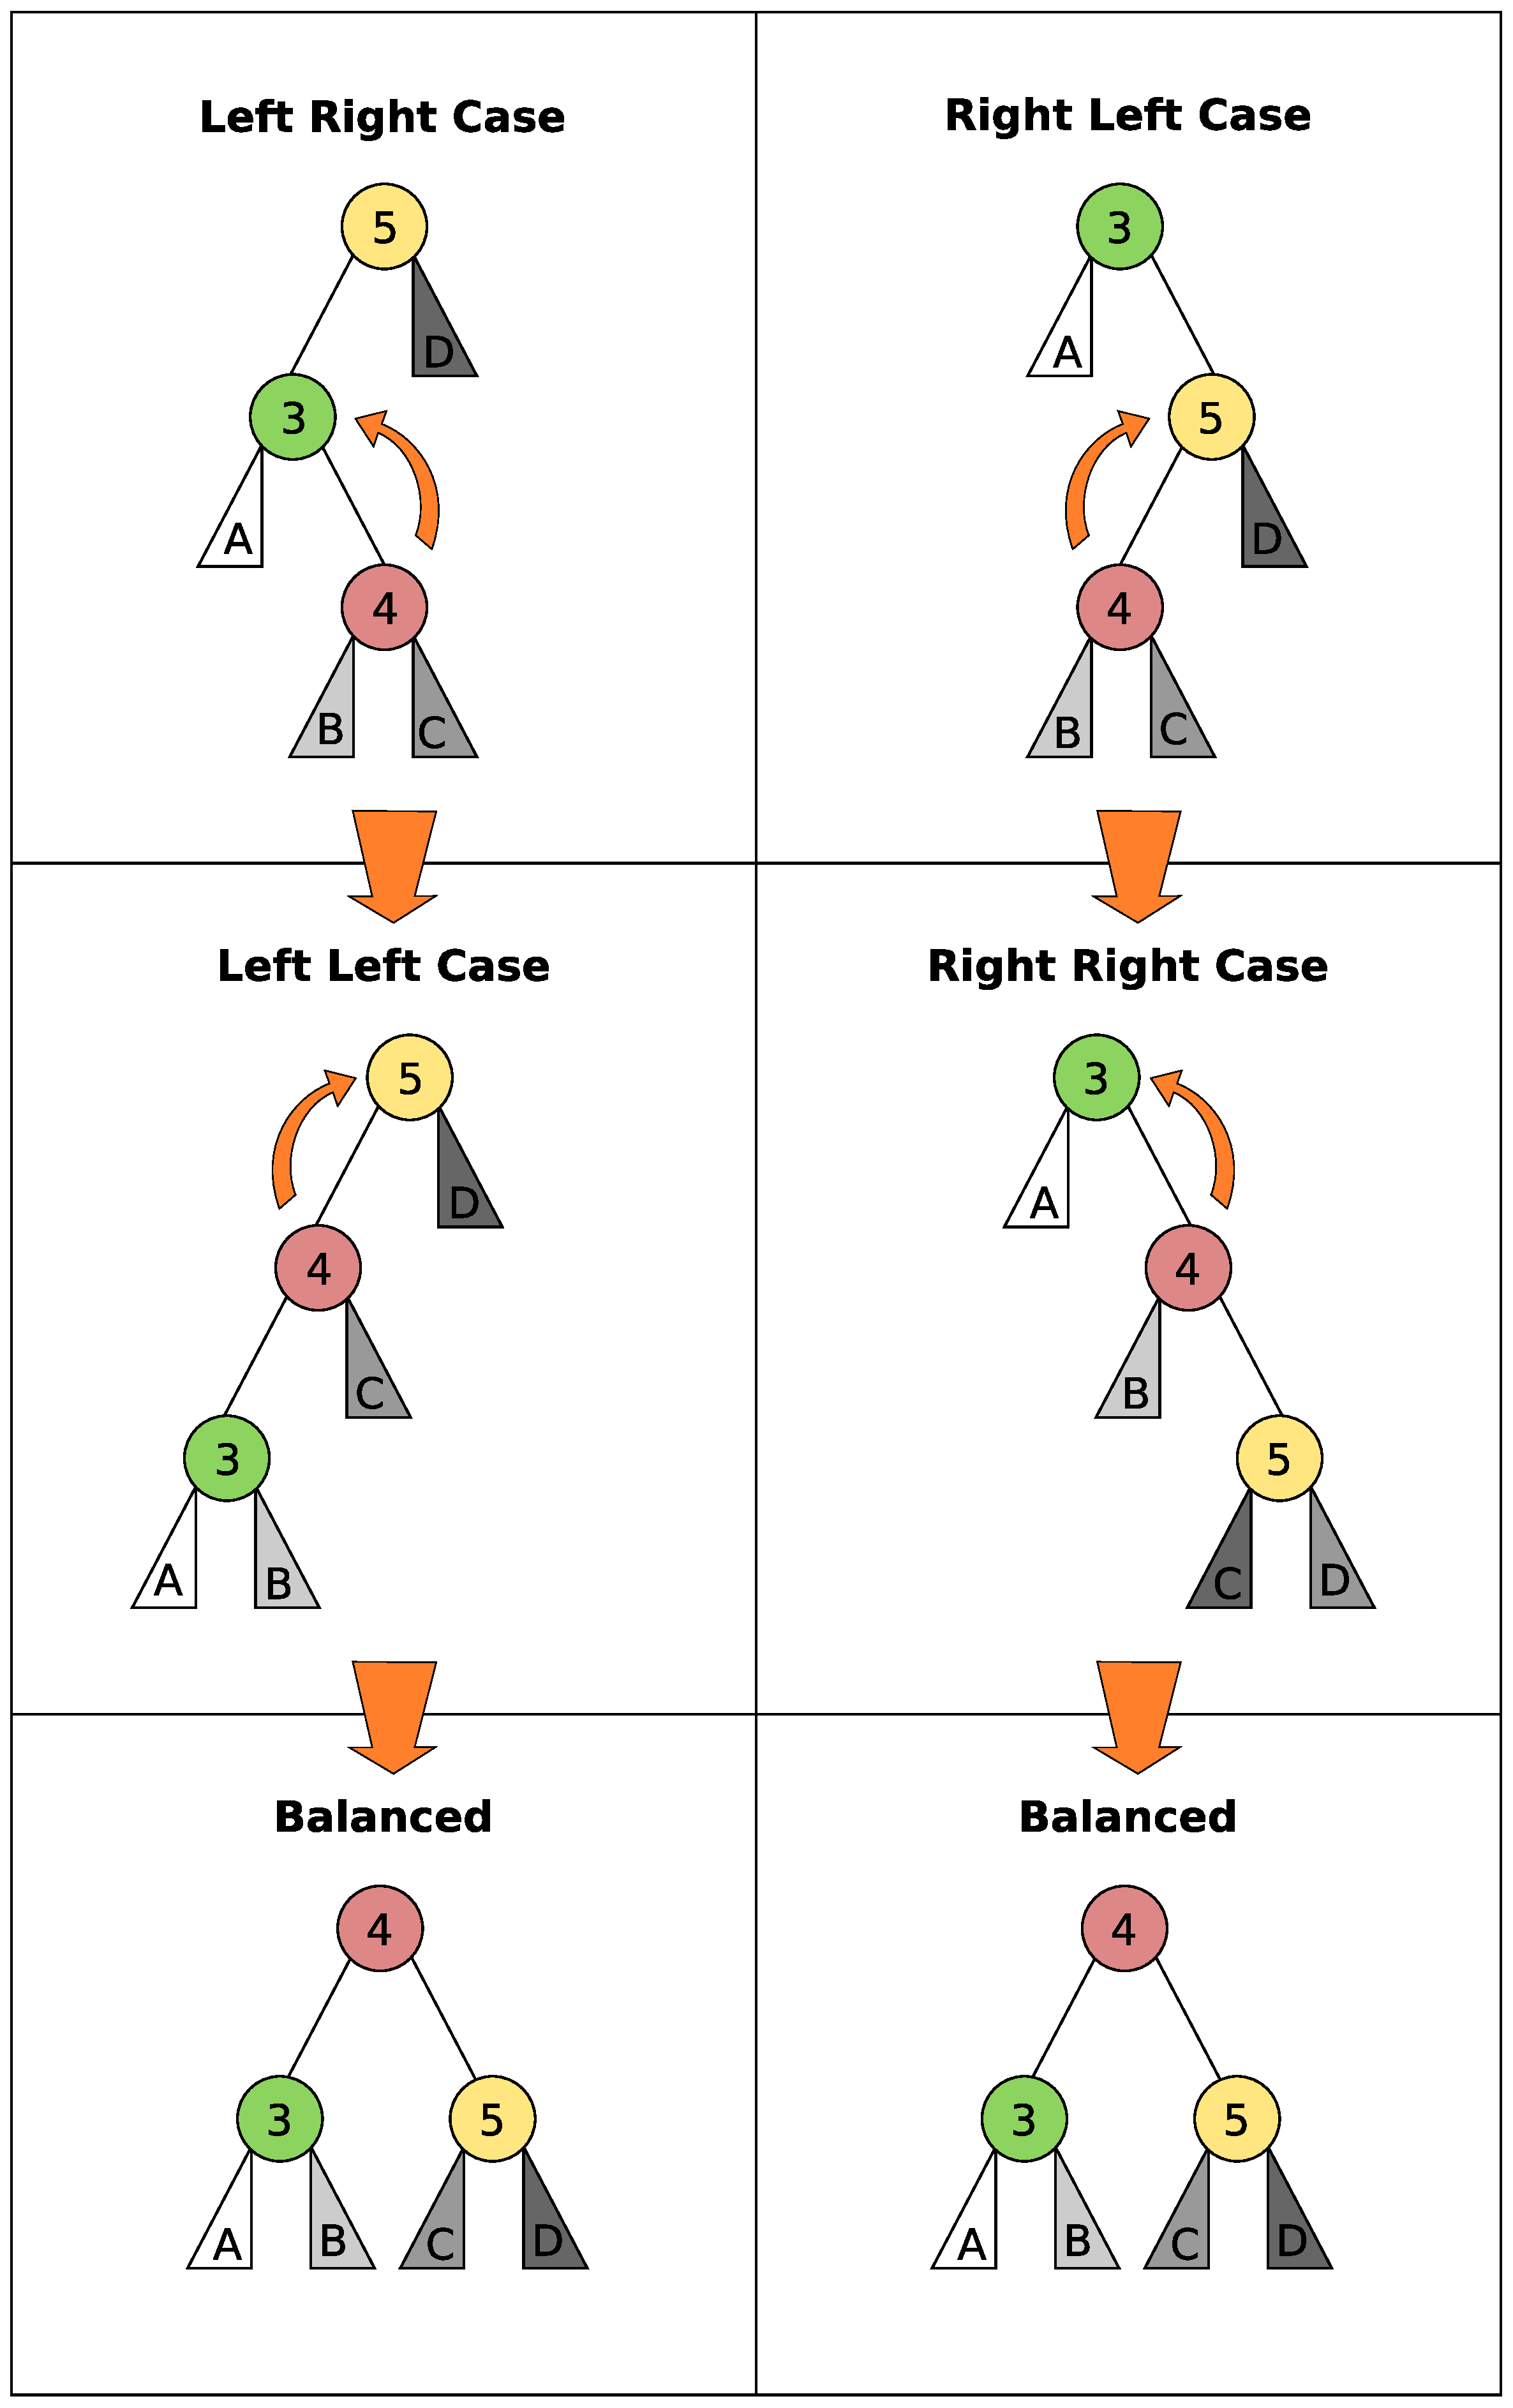
\includegraphics[height=16cm]{chapter13/AVL_Tree_Rebalancing.eps}
		%\begin{figure}
		%\centering
		%\def\svgwidth{\columnwidth}
		%\includegraphic{AVL_Tree_Rebalancing.eps}
		%\end{figure}

	\item	the procedure $\proc{AVL-Insert}(x, z)$ consist of $\proc{BST-Tree-Insert}(T, z)$ and $\proc{Balance}(x)$
	\item	$\proc{BST-Tree-Insert}(T, z)$: $\mathcal{O}(\log{n})$ \\
		$\proc{Balance}(x)$: $\mathcal{O}(\log{n})$ \\
		$\proc{AVL-Insert}(x, z)$ Total: $\mathcal{O}(\log{n})$
\end{enumerate}

